\section{目的}
依 PDF 88--90 頁實作 Lab 22 的4-to-1 multiplexer，完成講義兩種架構並設計較快TG版本，測量負載對延遲及能量的影響。

\section{Spec 對照}
S 表示已執行模擬檢查，D 表示分析與討論。

\small\begin{longtable}{p{.46\linewidth}p{.30\linewidth}p{.15\linewidth}}\toprule
要求與 PDF 頁碼 & 對應 deck／檢查 & 狀態 \\ \midrule\endhead
圖22.3 TG與static CMOS、10fF（88--89） & D01; D02/C0 & S \\
Delay、power、元件數比較（89） & D02; source probes & S+D \\
設計更快TG MUX（89） & Wide unbuffered tree & S; data path \\
三種MUX對load關係（90） & D02; 1--500fF & S \\
完整4-to-1真值表 & D01; 64 codes & S \\
\bottomrule\end{longtable}\normalsize


\section{電路與設計推導}
\[Y=\overline S_1\overline S_0A_0+\overline S_1S_0A_1+S_1\overline S_0A_2+S_1S_0A_3.\]
講義TG架構每一路有輸入inverter與兩個串聯TG，最後共用輸出inverter；static版本用四個NAND3和一個NAND4。新版本將四輸入排成兩層TG二元樹，六個TG均用8倍寬度，直接驅動輸出，沒有輸出inverter。全部 $L=0.25\,\mu$m，單位 $W_p/W_n=3.6/1.8\,\mu$m；NAND堆疊NMOS按串聯數等比加寬。每一架構另有兩個select inverter。新版本缺少增益恢復，依賴上游資料驅動，不可把小元件數等同小總面積。

為避免無緩衝TG的供應功率低估，於三種架構的每個資料輸入插入0 V電流探針，另外量資料源輸入能量。Supply+data仍不含理想select源的能量，也沒有建模上游實際driver。

\section{模擬設定}
模型由使用者於本機另行提供；採 1 V、27 $^\circ$C 的教學適配條件，不把講義舊製程的 2.5 V 數值視為本次通過門檻。使用 PrimeSim HSPICE S-2021.09、\texttt{accurate}、\texttt{runlvl=5}，由實際 \texttt{.print/.measure} 數據繪圖。每個 \texttt{.alter} 重設全部基準參數與溫度。所有案例皆完成，無 error 或 failed 量測；這不代表完全沒有模型或收斂提示。公開 netlist 僅保留 \texttt{* MODEL\_SETUP\_REQUIRED} 註解，不附模型路徑。完整數據位於該 lab 的 \texttt{results/}，大型資料依 deck 分檔，由 \texttt{simulation\_data.json} 索引。兩份deck共六案例。D01枚舉全部64組資料／選擇組合，每組2 ns，以每組80\%時刻檢查三輸出；0/1門檻為0.1/0.9 V。D02固定select=00，A0以20 ps邊緣、10 ns週期切換，分別掛1/10/50/100/500 fF，最大步距1 ps。Delay為A0到輸出的50\% crossing，非select路徑最壞delay。

\section{結果與規格檢查}
\begin{center}\small\begin{tabular}{lrrr}\toprule
Architecture & MOS core/all & $t_{rise}$ (ps) & $t_{fall}$ (ps) \\ \midrule
Lecture TG & 26/30 & 381.86 & 560.61 \\
Static CMOS & 32/36 & 230.90 & 364.48 \\
Wide TG tree & 12/16 & 52.16 & 92.85 \\
\bottomrule\end{tabular}\end{center}
\begin{center}\small\begin{tabular}{lrrr}\toprule
Architecture & $P_{supply}$ ($\mu$W) & $P_{data}$ ($\mu$W) & $P_{sum}$ ($\mu$W) \\ \midrule
Lecture TG & 23.886 & 2.943 & 26.829 \\
Static CMOS & 19.060 & 2.311 & 21.371 \\
Wide TG tree & -1.720 & 66.417 & 64.698 \\
\bottomrule\end{tabular}\end{center}
\begin{center}\small\begin{tabular}{lrrr}\toprule
Load (fF) & TG max (ps) & CMOS max (ps) & Tree max (ps) \\ \midrule
10 & 560.61 & 364.48 & 92.85 \\
1 & 507.14 & 348.69 & 90.62 \\
50 & 692.41 & 413.43 & 103.46 \\
100 & 799.99 & 474.38 & 116.16 \\
500 & 1586.69 & 1426.36 & 208.96 \\
\bottomrule\end{tabular}\end{center}

\begin{figure}[htbp]\centering
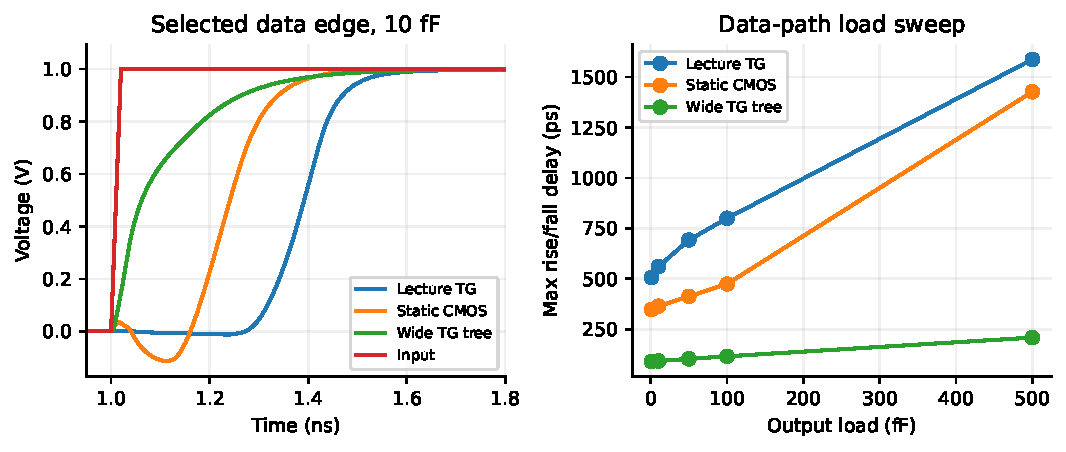
\includegraphics[width=\linewidth]{figures/mux_delay_load.pdf}
\caption{10 fF資料路徑與負載掃描；TG樹更快，但輸入源必須直接提供輸出充電電流。}
\end{figure}

\begin{figure}[htbp]\centering
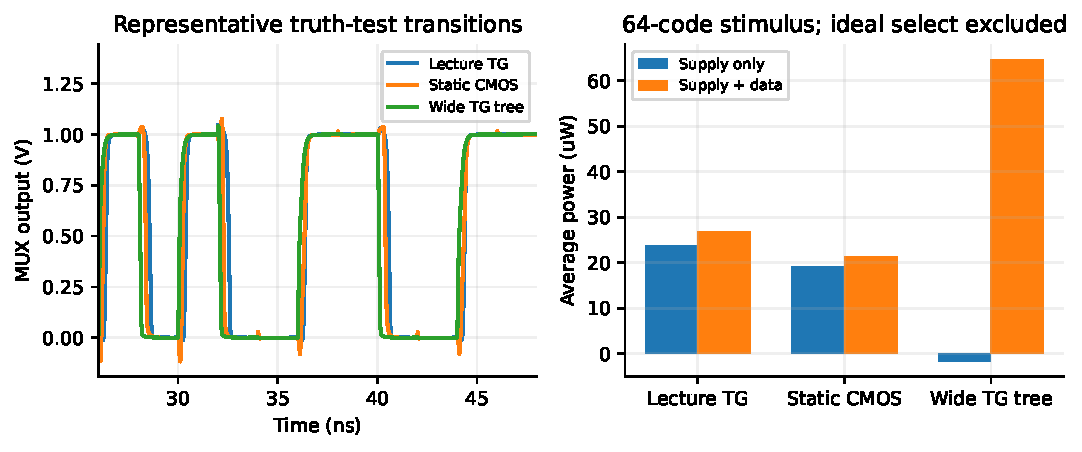
\includegraphics[width=\linewidth]{figures/mux_function_power.pdf}
\caption{代表性真值表轉態與64-code stimulus的功率。負的供應功率表示淨回灌，不是負的總消耗。}
\end{figure}
三種架構64/64組真值表全通過。10 fF下新TG樹rise/fall為52.16/92.85 ps，小於static CMOS的230.90/364.48 ps，完成指定資料路徑的速度目標。真值表stimulus下供應+資料功率卻為64.70 $\mu$W，高於CMOS的21.37 $\mu$W；不能把供應端-1.72 $\mu$W單獨當作省電結論。

\section{討論}
寬TG降低通道電阻、移除中間inverter減少門延遲，但增大資料與選擇端電容；直接輸出的能量由上游資料源提供。若接有限驅動器、長互連或大量MUX串接，速度優勢可能變小且需要再生buffer。Static CMOS提供增益恢復與明確邏輯驅動；原TG型有兩個再生inverter但多兩段傳輸延遲。負載增加時三種延遲皆增加，排序只適用於此尺寸與輸入條件。

波形中切換glitch與超軌尖峰保留，沒有用穩態真值表抹去動態hazard。此處元件數不包括stimulus、負載與量測源，且寬度不同，所以不能用晶體管數直接比較版圖面積。

\section{結論}
講義架構、較快TG改版、完整真值表及五種負載皆已驗證。較快的資料路徑以更高輸入能量與缺少邏輯再生為代價，不代表所有路徑或完整系統均最優。
